\section{A common question across Web learning and ranking-and-selection}

An item can be attractive because its permanent quality is high, because a persistent event temporarily raises demand, or because a shared platform shock affects many items. A measurement mixes these effects. Its usefulness depends on the decision: earning reward now, predicting a later reward, learning the best long-run alternative, or making a correct final selection. A graph can constrain permanent differences, correlate innovation noise, or do both. Treating these mechanisms as interchangeable obscures both the regret comparator and the information in a reading.

On the Web, navigation and co-engagement graphs arise naturally, while observations of detailed engagement or downstream opportunities can be selectively available. Our application interpretation is budgeted attention monitoring and opportunity selection. Recorded attention is an exogenous utility proxy; it does not measure the incremental engagement caused by displaying or promoting an item. This distinction is essential when interpreting offline panels.

The research began with similarity-based ranking and selection and developed along two streams. The graph stream asks how a supplied restriction eliminates statistically difficult alternatives and when graph construction is accurate enough to justify pooling. The temporal stream asks how sampling loses or preserves predictive information when unobserved arms continue evolving. Their combination retains fixed unknown means and a joint spatial innovation distribution, while allowing general, heterogeneous AR orders.

This document is a full research manuscript and evidence collection for later reduction. It includes the current mathematical results, algorithm definitions, experiments, negative findings, and application limitations. Appendices preserve complete technical derivations rather than omitting them for a conference page limit. An evidence manifest fingerprints the source versions used in the collection.

\subsection{Results and assumptions at a glance}
\begin{center}\small
\begin{tabular}{>{\raggedright\arraybackslash}p{.25\textwidth}>{\raggedright\arraybackslash}p{.32\textwidth}>{\raggedright\arraybackslash}p{.33\textwidth}}
\toprule
Result & What is established & Main condition \\
\midrule
Joint innovation likelihood & Exact predictable experiments and adaptive mean information & Known stable AR parameters, correct covariance/noise \\
Mean confidence and stopping & All-time contrast bounds and correct stopped recommendation & Fixed graph, supplied norm/energy bounds \\
Mean-UCB regret & Conservative sublinear mean pseudo-regret & Same assumptions, coverage probes \\
Current-state oracle floor & Positive expected linear innovation coefficient & Stationary Gaussian model, nondegenerate innovation contrasts \\
Graph information geometry & General design, resistance sensitivity, path--clique separation & Trusted graph-energy class; iid Gaussian information calculation \\
Selection formulas & Exact fixed-design Gaussian PCS and special allocation optima & Specific clock, prior, gap and observation conditions \\
Practical sampling & Mean, state, predictable-state and contrast rules & UCB/TS variants without a general optimality claim \\
Web data & Temporal modelling and topology controls on KuaiRec and Wikipedia & Exploratory selective-observation emulation \\
\bottomrule
\end{tabular}\end{center}

The current guarantees do not establish optimal restless control, sharp general graph-dependent temporal constants, learned-parameter confidence, or a universally best policy. These are meaningful future questions, rather than conditions silently assumed satisfied by the applications.

\section{Relation to existing theory}

Classical bounded stationary stochastic bandits have minimax regret of order $\sqrt{NT}$ for $T\ge N$, and important families have algorithms matching fixed-instance asymptotic information lower bounds~\cite{collected20,collected21,collected22}. A useful dependency model therefore restricts the alternatives the learner must distinguish, changes the information per observation, or changes the objective. It does not improve an unrestricted classical problem merely by smoothing estimates.

Spectral bandits and graph pure exploration already use graph-smooth reward means~\cite{collected1,collected17,collected2}. Clustered bandits already connect width and separation to regret~\cite{collected18,collected19}. Structured-bandit information programs and effective-resistance experimental design are established tools~\cite{collected11,collected24}. Our graph stream specializes them to quantitative energy restrictions, graph geometry and cumulative decisions. Its candidate incremental contribution is the explicit information sensitivity and a geometry-dependent achieved separation, not the general idea that similar arms share information. The original spectral selection index and its Operations Research follow-up motivate this question in ranking-and-selection~\cite{collected14,collected15,collected16}.

Time-varying Gaussian-process bandits already combine spatial and temporal kernels~\cite{collected3}. Shared linear-Gaussian and latent-AR bandits already use one action to learn about other actions and future rewards~\cite{collected4,collected5}. Predictive Sampling studies the remaining lifetime of information~\cite{collected10}; knowledge gradient studies the value of information for later decisions~\cite{collected6,collected30}. General AR processes become linear state-space models after stacking lags. Consequently, the joint filter itself is established machinery~\cite{collected33}. Our synthesis emphasizes the distinction between deterministic permanent-mean structure and correlated transient noise, adaptive likelihood under general orders, and sampling rules matched to different objectives.

Feedback graphs are a different observation model: they reveal neighbours' outcomes after a pull. Here an edge supplies a statistical restriction or covariance, and a pull directly reveals only selected coordinates. Neither the graph nor the filter manufactures additional observations. Full publication priority for each specialization remains unestablished; the original novelty audit is preserved in the evidence directory.

\section{Fixed means, restless rewards and two graph roles}

There are $N$ arms with deterministic unknown means $\mu_i$. Before observing the current field, select $a_t$ and receive
\begin{equation}
X_{i,t}=\mu_i+z_{i,t},\qquad
z_{i,t}=\sum_{r=1}^{p_i}a_{i,r}z_{i,t-r}+\eta_{i,t},\qquad
Y_t=X_{a_t,t}+\xi_t.
\label{eq:mainmodel}
\end{equation}
The innovations satisfy $\eta_t\stackrel{\mathrm{iid}}\sim N(0,Q_\eta)$, $Q_\eta\succ0$, while independent observation noise has variance $r\ge0$. AR polynomials are stable. All arms evolve every calendar time, whether sampled or not. For the theoretical results, orders, coefficients, innovation covariance, observation noise and stationary initialization are known.

Put $c_i=1-\sum_ra_{i,r}$. The raw AR intercept is $c_i\mu_i$, not $\mu_i$. Means are not regenerated between repeated-noise experiments. Algorithmic Gaussian draws represent uncertainty at a fixed truth. Some older special-case results explicitly average over a Gaussian prior; they are separately marked in the appendices.

Let $L_\mu$ be a candidate mean Laplacian and impose, when justified,
\begin{equation}
\mu^\top L_\mu\mu\le S^2,\qquad \|\mu\|_2\le B.
\end{equation}
This is deterministic side information. Independently, an innovation graph can supply a covariance such as a rescaled inverse of $\alpha_\eta I+\lambda_\eta L_\eta$. One graph may serve both roles, but that is an additional substantive assumption. Shared noise alone cannot identify the mean of an arm that never appears in the measurement design: the likelihood has no column for that mean. Mean regularization needs its own justification.

\subsection{The full lag process}
Stack lag deviations into $s_t$ and write
\begin{equation}
s_{t+1}=Fs_t+E\eta_{t+1},\qquad z_t=Cs_t,\qquad
\Gamma=F\Gamma F^\top+EQ_\eta E^\top.
\end{equation}
The stationary node-time covariance is
\begin{equation}
G_h=CF^h\Gamma C^\top,\qquad
(G_h)_{ij}=(Q_\eta)_{ij}\sum_{k\ge0}\psi_i(k+h)\psi_j(k),\quad h\ge0,
\end{equation}
where $\psi_i$ is the impulse-response sequence. Reverse-time covariances are transposes. Heterogeneous AR filters generally make $G_h$ asymmetric for positive lags and prevent a separable spatial-times-temporal kernel. A lag-20 process can have no one-period correlation but substantial dependence twenty periods later.

\subsection{Comparators must be fixed before designing a policy}
Let $b^*=\argmax_i\mu_i$. Four regrets are distinct:
\begin{align}
R_{\rm current}(T)&=\sum_t[\max_iX_{i,t}-X_{a_t,t}],\\
R_\mu(T)&=\sum_t[\mu_{b^*}-\mu_{a_t}],\\
R_{\rm stationary}(T)&=T\mu_{b^*}-\sum_tX_{a_t,t},\\
R_{\rm fixed}(T)&=\sum_t[X_{b^*,t}-X_{a_t,t}].
\end{align}
The first two are nonnegative pathwise. The latter two may be negative because adaptive decisions exploit predictable positive deviations. Under stationary initialization,
\begin{equation}
\E R_{\rm stationary}=\E R_{\rm fixed}
=\E R_\mu-\sum_t\E z_{a_t,t}.
\end{equation}
Terminal PCS is $\Pr(\widehat b_T=b^*)$ over repeated noise at a fixed truth. It is not the probability of finding the largest last reward. Pure exploration can spend reward to resolve a difficult permanent contrast, while a tracking policy can earn high actual reward from an arm with a lower permanent mean.

\section{Graph estimation using the correct trajectory likelihood}

For a fixed sampling schedule, let $M$ select the observed coordinates and $\Xi$ be their joint AR covariance including measurement noise. Then $Y\sim N(M\mu,\Xi)$ and
\begin{equation}
\mathcal I=M^\top\Xi^{-1}M,\quad q=M^\top\Xi^{-1}Y,\quad
\widehat\mu_H=(\mathcal I+H)^{-1}q,\qquad H=\alpha I+\lambda L_\mu.
\end{equation}
Spatial smoothness enters estimation through $H$; the graph-correlated AR likelihood enters through $\Xi$. Ignoring either changes the inference problem.

For a deterministic design and penalty, with $J=\mathcal I+H$,
\begin{equation}
\E\widehat\mu_H-\mu=-J^{-1}H\mu,\qquad
\Var(\widehat\mu_H)=J^{-1}\mathcal I J^{-1}.
\end{equation}
Inverse penalized information is not the repeated-noise covariance of a biased estimator. With $H=\lambda L_\mu$, the graph-energy bias of contrast $v$ is bounded by
\begin{equation}
\lambda S\sqrt{v^\top J^{-1}L_\mu J^{-1}v}.
\end{equation}
The common offset is unpenalized by a Laplacian. A proper $\alpha I$ regularizer is used for adaptive confidence.

An energy-constrained estimator literally imposes $\nu^\top L_\mu\nu\le S^2$. If its constraint is active, KKT gives
\begin{equation}
\widehat\mu_S=(\mathcal I+\lambda_*L_\mu)^{-1}q,
\qquad \widehat\mu_S^\top L_\mu\widehat\mu_S=S^2.
\end{equation}
Energy decreases monotonically along the positive multiplier, allowing a scalar search. Enforcing an estimate's radius does not establish that the unknown truth satisfies that radius. Same-data tuning of the graph or multiplier needs an uncertainty argument beyond fixed-penalty Gaussian calculations.

\subsection{Adaptive actions require predictable innovations}
Before time $t$, conditional on a candidate fixed $\mu$, maintain
$s_t\mid\mu,\mathcal H_t\sim N(g_t+D_t\mu,P_t)$. With $\ell_a=C^\top e_a$, define
\begin{equation}
v_{t,a}=e_a+D_t^\top\ell_a,\qquad d_{t,a}=\ell_a^\top P_t\ell_a+r,\qquad u_{t,a}=v_{t,a}/\sqrt{d_{t,a}}.
\end{equation}
The selected normalized observation is exactly
\begin{equation}
R_t=\frac{Y_t-\ell_{a_t}^\top g_t}{\sqrt{d_{t,a_t}}}
=u_t^\top\mu+\epsilon_t,\qquad \epsilon_t\mid\mathcal H_t,a_t\sim N(0,1).
\label{eq:maininnovation}
\end{equation}
Gaussian conditioning updates the affine mean and covariance, and propagation uses $F$. The designs $u_t$ are predictable even under adaptive actions. Thus
$\mathcal I_T=\sum_tu_tu_t^\top$ and $q_T=\sum_tu_tR_t$ match the recorded-path dense likelihood. This is an algebraic equality; it does not make an adaptively selected schedule an independent fixed design.

\section{Confidence, stopping, and stationary mean regret}

\begin{theorem}[Fixed-mean all-time contrast confidence]
Assume the correct known model, a graph fixed before measurement, $\mu^\top L_\mu\mu\le S^2$, $\|\mu\|\le B$, and $H=\alpha I+\lambda L_\mu\succ0$. With $J_T=H+\mathcal I_T$ and
\begin{equation}
\beta_T=\sqrt{\log\frac{\det J_T}{\det H}+2\log(1/\delta)}
+\sqrt{\alpha B^2+\lambda S^2},
\end{equation}
with probability at least $1-\delta$, simultaneously for all times and contrasts,
\begin{equation}
|v^\top(\widehat\mu_T-\mu)|\le\beta_T\sqrt{v^\top J_T^{-1}v}.
\end{equation}
\end{theorem}
\begin{proof}
The Gaussian innovation score $W_T=\sum_tu_t\epsilon_t$ admits the exponential martingale for every fixed vector. Mixing it with $N(0,H^{-1})$ yields
$\sqrt{\det H/\det J_T}\exp(\|W_T\|_{J_T^{-1}}^2/2)$. A crossing bound supplies the log-determinant term. The regularization contribution in $\widehat\mu_T-\mu=J_T^{-1}(W_T-H\mu)$ is bounded by $\sqrt{\mu^\top H\mu}$. Contrast Cauchy--Schwarz completes the result. The Gaussian mixing variable is a proof device, not a prior on the physical means.
\end{proof}

Stop and recommend $b=\argmax_i\widehat\mu_i$ only when every comparison exceeds its contrast width. The probability of an incorrect stopped recommendation is then at most $\delta$. A forced budget-terminal recommendation without passing the certificate has no such guarantee.

Let $A_i(e^{-\mathrm i\omega})$ be the AR polynomial on the unit circle and define
$a_{\min}=\min_{i,\omega}|A_i|$, $a_{\max}=\max_{i,\omega}|A_i|$. Put
\begin{equation}
v_-={\lambda_{\min}(Q_\eta)}/{a_{\max}^2}+r,
\qquad v_+={\lambda_{\max}(Q_\eta)}/{a_{\min}^2}+r.
\end{equation}
For every recorded schedule,
\begin{equation}
v_+^{-1}\diag(N_i(T))\preceq\mathcal I_T\preceq v_-^{-1}\diag(N_i(T)).
\end{equation}
These conservative spectral bounds permit consistency with growing coverage.

\begin{theorem}[Conservative certified mean-UCB bound]
After one initial reading of each arm, force cyclic probes at square calendar ages, with total forced count $F_T\le N+\sqrt T$. On other rounds select the largest $\widehat\mu_i+\beta\sqrt{(J^{-1})_{ii}}$. On the simultaneous event,
\begin{equation}
R_\mu(T)\le2BF_T+4\beta_T\sqrt{v_+NT},
\qquad
\beta_T\le\sqrt{N\log(1+T/(\alpha v_-))+2\log(1/\delta)}
+\sqrt{\alpha B^2+\lambda S^2}.
\end{equation}
For fixed dimensions and stable parameters this is sublinear.
\end{theorem}
\begin{proof}
Optimism bounds an ordinary action gap by twice its mean width. After initial coverage, $(J^{-1})_{ii}\le v_+/N_i$. Summing inverse square-root counts bounds ordinary regret by $4\beta_T\sqrt{v_+NT}$. Forced gaps are at most $2B$. The information upper bound and $H\succeq\alpha I$ bound the determinant.
\end{proof}
The expectation adds $2BT\delta$. A horizon-specific choice $\delta=1/T$ bounds that remainder. The experiment's practical UCB coefficient differs from the certified coefficient; a theorem for the latter must not be assigned to the former. This guarantee is conservative and does not give the sharp spatial or temporal regret coefficient.

\section{Graph alignment changes the alternative class}

Graph correctness has a quantitative meaning: a supplied restriction on means is actually true. Graph usefulness depends on the difficult alternatives that remain. Ordinal agreement or a lower smoothness quotient does not imply safe smoothing or a smaller regret constant for every policy.

Effective resistance gives
$|\mu_i-\mu_j|\le S\sqrt{(e_i-e_j)^\top L^\dagger(e_i-e_j)}$. This converts an energy radius into a component width. Certified pooling can then reject an entire suboptimal component when its uncertainty and supplied width are below its gap. Incorrectly small widths can remove the best arm and cause linear regret. Enlarging a valid certificate is safe but can remove most of the benefit.

\subsection{An exact graph-energy information design}
Consider a homogeneous suboptimal component of $m$ arms, gap $\Delta_c$, iid Gaussian observation variance $\sigma^2$, and supplied energy radius $S$. Let $s=S/\Delta_c$ and
\begin{equation}
F_L(p,s)=\min_i\min_{\substack{z\in[0,1]^m,\ z_i=1\\z^\top Lz\le s^2}}\sum_jp_jz_j^2,
\qquad F_L^*(s)=\max_{p\in\Delta_m}F_L(p,s).
\end{equation}
The structured information program gives component constant
\begin{equation}
C_{L,S}=\frac{2\sigma^2}{\Delta_cF_L^*(S/\Delta_c)}.
\end{equation}
For a fixed graph, $F_L^*$ decreases as the supplied uncertainty expands, lies in $[1/m,1]$, and equals one at zero energy. A finite-strength resolvent $(\diag(p)+\tau L)^{-1}$ solves the inner quadratic optimization. This connects the original spectral index with an information calculation; it is not itself a regret theorem for choosing the largest smoothed value.

Define the resistance radius
\begin{equation}
\rho_L=\min_{p\in\Delta_m}\max_i\sqrt{(e_i-p)^\top L^\dagger(e_i-p)}.
\end{equation}
It equals the radius of the minimum enclosing ball in the effective-resistance embedding, an established geometric object. Its local information sensitivity is
\begin{equation}
\frac{C_{L,S}}{2\sigma^2/\Delta_c}
=1+2(S/\Delta_c)\rho_L+O((S/\Delta_c)^2D),
\end{equation}
where $D$ is the resistance diameter. The radius, rather than diameter alone, sets the first-order price of the supplied uncertainty.

\subsection{A path--clique separation and an achieved policy result}
A clique with edge weight $1/m$ and a path with weight $(m-1)/2$ have resistance diameter two. At $S=\Delta_c$, every clique coordinate can independently become optimal, giving $C_{\rm clique}=2\sigma^2m/\Delta_c$. A half-and-half endpoint design on the path gives
\begin{equation}
C_{\rm path}\le\frac{2\sigma^2}{\Delta_c(1-1/\sqrt2)^2},
\end{equation}
which has no factor $m$. Identical component diameters therefore conceal a growing information separation.

Graph-design elimination with UCB fallback uses a preselected resistance design, valid energy allowances, capped stages and ordinary-arm fallback. Its proved finite-time result protects the optimal component and attains logarithmic regret without linear component-size dependence on the normalized path. It is not proved to match the exact information constant on general positive-uncertainty classes. Small-instance pilot overhead can make it substantially worse than ordinary UCB.

Certified Laplacian error also has an explicit price. If $(1-\zeta)L\preceq\widehat L\preceq(1+\zeta)L$, a radius $S$ under $L$ is safely enlarged to $\sqrt{1+\zeta}S$ under $\widehat L$. This repairs the mean restriction when the likelihood remains correct. It cannot repair a covariance likelihood fitted from the wrong graph.

\section{Combining pooling with persistent observations}

An innovation-regression confidence set permits certified component bounds even when observations are correlated over space and time. For a component $C$, a supplied diameter $\varepsilon_C$, estimate $m$, inverse information $V$, and confidence coefficient $\beta$, define
\begin{equation}
U_i=m_i+\beta\sqrt{V_{ii}},\qquad
U_C=\min\left\{\max_{i\in C}U_i,
\min_{w\in\Delta(C)}(w^\top m+\beta\sqrt{w^\top Vw})+\varepsilon_C\right\}.
\end{equation}
On the all-contrast event, both terms upper-bound the largest permanent mean in $C$. A selected suboptimal component with gap $\Delta_C>\varepsilon_C$ must satisfy
\begin{equation}
\min_{w\in\Delta(C)}w^\top Vw
\ge\frac{(\Delta_C-\varepsilon_C)^2}{4\beta^2}.
\end{equation}
This is a valid realized-information rejection condition. Converting it into a count-based regret formula needs an information-growth condition for the actual schedule. The spatially correlated case does not inherit an arbitrary per-pull constant from a full-field experiment.

\subsection{Two corrections needed when reusing the bridge notes}
The collected bridge notes contain proposed extensions, not a blanket new theorem. First, with independent-arm AR(1), one pull adds at least $(1-\phi)^2/(V+r)$ information to that arm under the stated positive-persistence filter conditions. The inverse variance of a pooled component depends on the \emph{sum} of arm information. Its per-pull increase has this same lower bound, not $|C|$ times that bound. A component-size factor requires $|C|$ scalar readings and must be charged accordingly.

Second, a simultaneous observation of a subset $S$ has innovation covariance $Q_{SS}$ and precision $(Q_{SS})^{-1}$. It does not generally have precision $(Q^{-1})_{SS}$: the latter conditions on the unobserved contemporaneous coordinates. For common coefficients and a continuously observed subset, the long-run comparison covariance is $Q_{SS}/c^2$, giving pair contrast variance $2q(1-\rho)/c^2$ in the equal-variance case. Arbitrary partial restless schedules need the exact conditional filter, rather than substitution of a full-field precision.

These corrections preserve the useful validity bridge while narrowing unverified information-growth claims. The main certified mean-UCB theorem does not rely on either incorrect factor.

\subsection{Persistence breaks iid confidence under bursty exposure}
For consecutive observations from stationary AR(1) with variance $V$,
\begin{equation}
\Var(\bar Y_n)=\frac Vn\left[\frac{1+\phi}{1-\phi}
-\frac{2\phi(1-\phi^n)}{n(1-\phi)^2}\right].
\end{equation}
An iid radius based on $V/n$ underestimates uncertainty. The limiting variance inflation is $(1+\phi)/(1-\phi)$. Widely separated UCB pulls may avoid much of this effect; bursty exposure reveals it. The coverage experiments report high iid miscoverage and erroneous irreversible elimination at strong persistence, whereas innovation-based certificates remain valid but can be so wide that they eliminate nothing. Correctness and the reward cost of that correctness must both be reported.

\section{Sampling rules for reward and permanent selection}

\subsection{Shared forecast and three uncertainty sources}
For past readings, define $K=\Cov(z_t,\text{selected past deviations})$, $A=K\Xi^{-1}$, $W=I-AM$, $V=(H+M^\top\Xi^{-1}M)^{-1}$ and $m=VM^\top\Xi^{-1}Y$. Then
\begin{equation}
f=AY+Wm,\qquad P=G_0-K\Xi^{-1}K^\top,\qquad \Sigma=P+WVW^\top.
\end{equation}
These working quantities distinguish uncertainty in fixed means, uncertainty about past lag states, and the current innovation. $\Sigma$ supports randomized decisions; frequentist confidence additionally includes regularization bias and adaptive uncertainty.

Mean UCB/TS acts on $m,V$. Full-state UCB/TS acts on $f,\Sigma$. Predictable-state UCB/TS acts on $f,\Sigma-Q_\eta$. The last matrix is positive semidefinite under the correct model because
\begin{equation}
z_t=CFs_{t-1}+\eta_t,
\qquad P-Q_\eta=\Var(CFs_{t-1}\mid\mathcal H_t,\mu)\succeq0.
\end{equation}
Removing fresh innovations retains learnable mean and past-state uncertainty. It can reduce futile randomized exploration. It remains a one-step heuristic and can undervalue delayed AR information. It is distinct from both future-information Predictive Sampling and the older KuaiRec mean-only perturbation rule.

All joint Gaussian perturbations preserve cross-arm covariance. Drawing independent arm marginals is an approximation and must be labelled. No standard linear-TS theorem is imported: the whitened design vector differs from the physical reward coordinate and changes with the history.

\subsection{Permanent-contrast allocation}
For contrast $v$ and a candidate normalized reading $u_{t,a}$, the exact reduction in inverse regularized information is
\begin{equation}
g_t(v,a)=\frac{(v^\top Vu_{t,a})^2}{1+u_{t,a}^\top Vu_{t,a}}
=\frac{(v^\top VW_{a,:}^\top)^2}{\Sigma_{aa}+r}.
\end{equation}
Contrast LUCB chooses a current best estimate and an optimistic challenger, then measures the arm maximizing this gain. Top-two Thompson contrast sampling draws plausible competing mean winners and uses the same gain. A third arm can best resolve their comparison. These are practical fixed-budget heuristics, not proved globally PCS-optimal allocations.

An observation's conditional reduction in a future target variance is
\begin{equation}
\Delta_{i,h}(a)=\frac{(e_i^\top CF^hP_t\ell_a)^2}{\ell_a^\top P_t\ell_a+r}.
\end{equation}
Replace $e_i$ by a contrast to value a future comparison. The entire impulse profile matters; one lag-one correlation coefficient is insufficient.

\subsection{What is the best policy in principle?}
With known parameters, the finite-horizon optimal policy solves the belief-state Bellman equation
\begin{equation}
J_h(b)=\max_a\{f_a(b)+\E[J_{h-1}(\mathcal T_a(b,Y_a))]\},\quad J_0=0.
\end{equation}
The state includes every mean and lag belief. Exactly two remaining decisions have a Gaussian knowledge-gradient score: immediate forecast plus the expected maximum of next forecasts after one observation. Independent arms admit a normal-density/CDF expression. In a joint graph state, one observation moves every next forecast, producing an expected maximum of correlated affine functions of one normal variable. Rolling that two-period score is feasible; it does not solve the general Bellman equation.

Long-horizon approximations can outperform Predictive Sampling at moderate persistence and lose at near-unit persistence. The optimality statements in the two-period and special selection theorems therefore do not imply a uniformly best indefinite-horizon sampling algorithm.

\section{Information limits and exact allocation cases}

\subsection{A linear floor against current-state information}
Let $\mathcal G(\mu,K)=\E\max_i(\mu_i+Z_i)$ for $Z\sim N(0,K)$. A genie seeing all past lag states and the true means has current conditional covariance $Q_\eta$. Its forecast field has covariance $G_0-Q_\eta$. Thus every causal policy's expected current-oracle regret satisfies
\begin{equation}
\E R_{\rm current}(T)\ge T\left[\mathcal G(\mu,G_0)-\mathcal G(\mu,G_0-Q_\eta)\right].
\end{equation}
Nondegenerate innovation contrasts make the coefficient positive. This is an expected floor, not a pathwise inequality, and generally not attainable with one selected reading per round. A known-mean greedy filter is a benchmark, not an optimal causal policy. For simultaneous $b$-arm sets replace the maximum by the sum of the largest $b$ coordinates and charge $bT$ measurements.

\subsection{Mean information and long-run covariance}
For noiseless full fields, with $p=\max_i p_i$ and $D_c=\diag(c_i)$,
\begin{equation}
\mathcal I_n=\mathcal I_p+(n-p)D_cQ_\eta^{-1}D_c,
\qquad \mathcal K_{\rm LR}=D_c^{-1}Q_\eta D_c^{-1}.
\end{equation}
Persistence can strengthen prediction while making permanent means harder to learn. In adaptive selected feedback,
\begin{equation}
\KL(P_\mu^{\pi,T},P_\nu^{\pi,T})
=\tfrac12\E_\mu[(\mu-\nu)^\top\mathcal I_T(\mu-\nu)].
\end{equation}
This identity yields comparison lower bounds by change of measure. It does not turn an arbitrary schedule into a consecutive full-field experiment.

\subsection{Two independent AR(1) means: exact schedules}
For exact stationary AR(1) observations separated by gaps $h_r$, variance $V$ and known $0\le\phi<1$,
\begin{equation}
I(\mathcal T_i)=\frac1V\left[1+\sum_{r=2}^{n_i}\frac{1-\phi^{h_r}}{1+\phi^{h_r}}\right].
\end{equation}
At fixed positive gap $\Delta$, fixed-schedule GLS comparison has PCS
$\Phi(\Delta/\sqrt{I_1^{-1}+I_2^{-1}})$. For even budget $T$, strict alternation is the optimal fixed calendar schedule, with per-arm information
\begin{equation}
I_*=\frac{T(1-\phi^2)+4\phi^2}{2V(1+\phi^2)}.
\end{equation}
Under the separate symmetric prior $\mu_i\sim N(0,\tau^2)$, alternation also attains the optimal prior-averaged adaptive PCS
$1/2+\arctan(\tau\sqrt{I_*})/\pi$. The prior-averaged theorem is not a uniform adaptive frequentist statement at every fixed pair.

For next-round terminal-state selection with known means, observing different arms in the last two rounds is adaptively optimal; older observations add no forecast information once exact latest states are known. The next-round PCS is
\begin{equation}
\frac12+\frac1\pi\arcsin\left(\phi\sqrt{(1+\phi^2)/2}\right).
\end{equation}
Changing the target to the last observed round changes the formula. This explains why large budgets can improve permanent identification without improving a particular terminal-state objective.

\subsection{General AR changes the allocation geometry}
For correlated lag-two processes $z_{i,t}=az_{i,t-2}+\eta_{i,t}$ with marginal variance $V$ and innovation correlation $\rho$, four-calendar-sample GLS contrast variances are
\begin{equation}
\sigma^2_{AABB}=V+r-a\rho V,\qquad
\sigma^2_{ABAB}=V+r+aV.
\end{equation}
At $V=1,r=.1,a=.8,\rho=.6,\Delta=.4$, PCS is .6943 versus .6142. Blocks reduce within-arm redundancy and access shared noise at informative lags. This is a strict comparison of two designs, not a universal four-step optimum.

For three or more arms, balanced information need not maximize Bayesian PCS. With heterogeneous AR, the latest observation is not generally a sufficient prediction summary. Exact multi-arm fixed-design PCS has a one-dimensional Gaussian integral, while adaptive designs require different probability arguments.

In separately advanced \emph{rested} AR streams, mean information becomes affine in the sample count after the initial lag block. With long-run variance constants $\kappa_i$, supplied gaps $\Delta_i$, and best arm $b$, the fixed-proportion error exponent is
\begin{equation}
E(w)=\min_{i\ne b}\frac{\Delta_i^2}{2(\kappa_b/w_b+\kappa_i/w_i)}.
\end{equation}
Its optimal proportions follow from one root
\begin{equation}
\frac{\kappa_b}{u^2}=\sum_{i\ne b}\frac{\kappa_i}{(\Delta_i^2-u)^2},\qquad
w_b\propto\kappa_b/u,\quad w_i\propto\kappa_i/(\Delta_i^2-u).
\end{equation}
This is an exact asymptotic allocation benchmark in that clock, not a finite-budget optimal policy for restless Web arms.

\section{Controlled numerical evidence}

\subsection{Fixed-truth 100-arm AR(20) study}
The primary controlled study uses a 10-by-10 graph, 100 arms, order twenty, 32 independent paired noise worlds per configuration, and 1,000 calendar decisions including initial coverage. Five configurations isolate persistent dense filters, weak dense filters, lag-20 seasonality, heterogeneous/oscillatory filters, and diagonal innovations. The same deterministic mean vector is used in every replicate and configuration; the top gap is .20. Stationary marginal deviation variance is one and sensor variance is .09.

Fourteen learning rules and four information benchmarks share innovation paths and potential sensor noises within a world. Practical UCB scale .7, Thompson scale one, $H=.1I+.5L$ and supplied bounds $B=6,S=3$ are fixed, not optimized by configuration. Numerical verification contains 642 assertions against dense likelihood, heterogeneous covariance orientation, independent filters and contrast gains; a recorded exact reproduction matches one complete world across all policies.

\begin{center}\small
\begin{tabular}{lrrrr}
\toprule
Configuration & IID UCB & Joint state UCB & Joint predictive UCB & Innovation floor \\
\midrule
Persistent & 1.397 & 1.248 & 1.426 & .493 \\
Weak & 2.131 & 1.838 & 2.008 & 1.556 \\
Lag twenty & 2.160 & 1.760 & 1.838 & .340 \\
Heterogeneous & 1.717 & 1.647 & 1.617 & .789 \\
Diagonal shocks & 1.453 & 1.270 & 1.491 & .515 \\
\bottomrule
\end{tabular}\end{center}
Entries are current-state-oracle regret per decision; the floor is separately estimated expected Gaussian regret. Full intervals and all methods are in Appendix~\ref{app:st} and the frozen result tables. State UCB beats IID UCB on these instances, but the predictive UCB rule is not uniformly better than full-state UCB or temporal-only UCB.

The objectives produce different leaders. In weak dependence, joint mean UCB has mean pseudo-regret .487 versus IID UCB .607; predictive UCB has PCS 29/32 = .906, with Wilson interval [.758,.968]. In lag-20 dependence, contrast LUCB has PCS 27/32 = .844 versus round robin 9/32 = .281; the paired difference is .5625 with interval [.339,.786]. Persistent dynamics make permanent selection harder even when immediate tracking improves.

Removing fresh noise from Thompson perturbations improves current-oracle regret over full-state TS by .043--.327 per decision across the five configurations, with positive paired pointwise intervals. It still need not beat other policy families. In the persistent instance, full-state UCB has stationary actual-reward regret $-.308$ per decision despite positive mean pseudo-regret .686. Tracking positive deviations explains this apparent reversal.

\subsection{Smaller general-AR and policy-control experiments}
Six-arm fixed-truth studies compare lag-two, oscillatory and heterogeneous order-two/order-three dynamics on smooth and rough mean vectors. Graph contrast allocation improves some smooth instances and loses on some rough instances. The exact AR(2) schedule formula is directly verified. These results illustrate mechanisms rather than uniform superiority.

Known-mean AR(1) control uses forty paired long-horizon worlds. At $\phi=.9$, two-period control has oracle regret .4334 per round, versus Predictive Sampling .5669 and lifetime-weighted knowledge gradient .4574. At $\phi=.99$, Predictive Sampling .1495 beats lifetime-weighted KG .1659 and two-period .1997. Near-unit persistence favours a longer useful-information horizon, but one-observation lifetime weighting is not an optimal Bellman continuation.

Two-arm allocation checks use 40,000 replications at budget ten and confirm the corresponding prior-averaged or terminal-state formulas within Monte Carlo uncertainty. For example, at $\phi=.9$, optimal mean Bayes-PCS is .67103 and optimal next-state PCS is .82717. Those experiments explicitly use a mean prior for the first target, unlike the fixed-truth AR(20) study.

\subsection{Alternative random-mean toy and coverage tests}
The separate toy benchmark samples a graph-correlated mean population, uses 100 grid arms, AR(20), eight seeds and 2,000 rounds. It is supplemental Bayesian evidence, not a fixed-mean replication of the primary experiment. Its joint predictable-state rule has oracle regret .950 versus IID TS 1.329 and temporal-only predictable sampling 1.121 in the persistent configuration. A UCB multiplier selected on the reported runs attains .850, but that selection has evaluation bias and must not become an independently tuned headline.

Coverage experiments compare iid pooling with the innovation certificate across persistence and block exposure. Under blocks of twenty-five and $\phi=.97$, iid certificates are violated in 90--100\% of runs; successive elimination removes the best arm in 65--75\% for some configurations. Certified methods show no violations in the reported runs but the conservative multivariate certificate often eliminates nothing at budget 5,000. A valid scalar certificate for independent shocks reduces the conservatism; it does not extend automatically to correlated designs. These are finite simulation frequencies, not a replacement for theoretical coverage statements.

\subsection{Graph geometry and invalid certificates}
The path--clique simulations measure the overhead of geometry-aware elimination as well as its eventual advantage. At component size 256, path graph-design elimination has regret about 46.08 versus ordinary UCB 191.83 in the reported experiment; at size sixteen it has 40.32 versus 10.81. On the clique it is worse than UCB at the smaller sizes. Geometry can reduce the arm-count dependence without guaranteeing a gain at every finite budget. Invalid-certificate stress tests demonstrate elimination errors and near-linear regret. Full parameter definitions, pointwise uncertainty and tables remain in Appendix~\ref{app:alignment}.

\section{KuaiRec: static structure and persistent engagement}

KuaiRec~\cite{kuairecdata} supplies both a nearly complete static user--video matrix and daily aggregate engagement. These are different observation experiments. The repository's raw data and scripts are local; application results below are the existing pilot evidence, preserved without rerunning or altering them.

\subsection{Static graph alignment and pooling}
Sixteen user/item graphs are assessed with mean-degree-normalized Laplacians and degree-preserving nulls. Co-engagement is the best user graph: smoothness quotient .649 against .791 for its rewiring. Item factorization and co-engagement carry personal-taste signal, whereas author, tag and category links mostly group popularity. The social graph covers only eighty evaluation users with forty-seven edges, insufficient for a broad social claim.

Mean-square smoothness is not safe-ranking evidence. Smoothing on real item graphs can change the best video more than smoothing on rewirings does. In 60-user, 300-video, 20,000-round bandit instances, strong spectral TS often helps the typical user but has heavy tails. Its median ratio to Bernoulli TS on I-mf is .68, while strong I-coeng smoothing has 90th-percentile ratio 18.78. Uncertified author pooling has 90th-percentile ratio 29.61. Oracle-certified pooling roughly halves UCB1 regret on some graphs, but the oracle diameter is supplied by the truth and is not a practical certificate.

Graph-free shrinkage is a necessary control. A rewired item graph matches real I-mf performance for spectral methods. In the 300-user by 100-video cold-user experiment, complete-graph shrinkage has mean regret ratio .726 to per-user TS versus .759 for co-engagement and .745 for its rewiring. Population shrinkage explains much of the gain. Energy certificates are typically too loose: the energy-to-gap ratio is about five. UCB-style comparisons also used a conservative noise proxy that disadvantages them against Bernoulli TS; new application comparisons must match variances or use appropriate KL indices.

\subsection{Daily engagement pilot}
The existing daily study uses 253 evaluation videos with records on all 63 dates, ten daily slots, full prefixes of 28, 35 or 42 days, pooled lags $\{1,2,7\}$, and five stochastic seeds. The reward is a transformed daily completion rate. Averaging origins gives:
\begin{center}\small
\begin{tabular}{lr}
\toprule Policy & Current-field regret per day \\
\midrule
ST greedy & 2.411 \\
Temporal-only greedy & 2.436 \\
Mean-only perturbation, graph & 2.630 \\
Mean-only perturbation, rewired & 2.635 \\
Mean-only perturbation, common shock & 2.615 \\
ST UCB & 2.742 \\
Last value & 2.883 \\
IID Gaussian TS & 3.902 \\
Full-current-state TS & 4.576 \\
Fit-window ranking & 4.906 \\
\bottomrule
\end{tabular}\end{center}
Temporal modelling is promising, while the incremental graph improvement over temporal greedy is only about 1\%. With substantial historical information, greedy is strong. The older mean-only perturbation rule is not the new $\Sigma-Q$ rule: it omits uncertain past-state deviations as well as fresh shocks. At the last origin, stale last value beats the fitted models, suggesting lifecycle drift beyond a fixed-mean stationary process.

\subsection{A chronology and missingness audit}
The newly executed audit finds 343,341 video-days, 10,728 videos and 63 dates, with no duplicate video-days. The 253-video complete-by-presence cohort has six zero-play cells on two videos. A pseudocount logit at zero plays has no observed completion-quality information.

The static graph pipeline excludes evaluation pairs, but it uses all interaction dates. At the earliest daily cutoff, 79.1\% of item-graph side-input rows occur later than the cutoff; the later origins still include 34.9\% and 24.9\% later rows. Consequently, the daily graph comparison cannot be treated as a leakage-free chronological result. The three windows overlap, and algorithm seeds do not create independent data fields.

The pilot remains useful exploratory evidence. A corrected replication must rebuild co-engagement, IDF and factors using only dated prefix interactions, distinguish missing/zero-play quality, and disclose any hindsight survivor cohort. It cannot infer exact permanent means, PCS or a stationary innovation floor from this short drifting panel. Those endpoints remain controlled-model measurements.

\section{A new laptop-sized Wikipedia experiment}
\label{sec:wiki}
The new application is selective monitoring of observed Web attention. A fixed topic catalog supplies opportunities with daily utility proportional to observed attention; inspecting selected articles reveals their current statistic. Public views are inexpensive, so the budget emulates a more costly downstream inspection rather than demonstrating measured production savings. No claim of promotion lift or causal click-through improvement is made.

\subsection{Data and historical graph}
Two panels are chosen before test retrieval: twenty-four astronomy/space articles and twenty-four football articles. Each has complete daily human-traffic page views from 1 January 2024 to 30 June 2025, obtained from Wikimedia's public API~\cite{wikiapi}. Titles, request URLs, raw responses and hashes are saved. The panel choices are a small purposive sample rather than representative Web content.

For each article, retrieve the final available revision dated no later than 31 December 2023 using the revisions API~\cite{wikihistory}. Extract direct hyperlinks to the other panel members and symmetrize their binary adjacency. No test attention, current link structure, or current redirect resolution enters the graph. This is a historical hyperlink graph, not a clickstream graph. A degree-preserving rewiring supplies a null with identical node degrees; its completed swap count is recorded. Neighbourhood structure may still poorly describe attention shocks.

The reward is $\log(1+\text{daily human views})$. All arms use the same transformation. No per-arm standardization is applied, since it would change the ranking task. Training-only weekday effects are subtracted during filtering and added back to decision scores. Raw-view opportunity loss is reported alongside transformed regret. A transformed long-run mean is not necessarily the raw-count mean.

\subsection{Fitting, feedback and budgets}
The primary dynamics are pooled general AR(7) with nonzero lags $\{1,2,7\}$, fitted by ridge regression. A dense AR(20) sensitivity tests the higher-order model. The first 274 days of 2024 fit preprocessing and dynamics; its remaining 92 days select covariance shrinkage settings by forward residual Gaussian score and practical UCB multipliers by development regret. After choosing these settings, parameters are refitted on all 366 days of 2024. No 2025 values select the configuration.

Innovation covariance is compared across a diagonal temporal-only model, a historical graph kernel plus common factor, the rewired kernel, a common-factor model and graph-free empirical-covariance shrinkage. Arm-specific innovation scales are shared across covariance families. Every covariance is positive definite. If an AR fit is unstable, an explicitly recorded absolute-sum constraint rescales its coefficients; the original radius and scale are reported. A $10^{-8}$ observation variance is a numerical regularizer, not injected synthetic feedback noise.

All learners receive the same full 2024 history. This mature-catalog initialization costs 8,784 historical scalar readings per panel and is disclosed separately from test observations. The joint filter appends a static mean with diffuse working Gaussian uncertainty to the AR lag state; these beliefs are algorithmic uncertainty at fixed physical means. Historical observations are assimilated once. There is no random mean population and no theorem transferred to the fitted real-data model.

The test is the continuous 181-day field from January through June 2025. Each day select one article or five distinct articles simultaneously, then reveal only those coordinates. A batch is chosen before any same-day feedback. There is no full-field test refresh and no overlapping test-origin replication. State dimensions are 192 for AR(7) and 504 for AR(20), small enough for exact covariance filtering on the laptop.

\subsection{Comparisons, endpoints and uncertainty}
The main comparison includes fit-history ranking, last observation, round robin, variance-matched iid UCB/TS, sliding-window UCB, temporal-only greedy and predictable-state UCB/TS, joint greedy, full-state UCB/TS, joint predictable-state UCB/TS, and predictable-state sampling with rewired, common-factor and graph-free covariance. Mean regularization is omitted to isolate innovation dependence. Thompson scale is fixed at one; UCB multipliers are selected from $.5,1,2$ on development data. Stochastic AR(7) methods use ten seeds; deterministic methods run once. AR(20) sensitivity uses three stochastic seeds and the matched UCB/TS pairs.

The evaluation oracle knows the current \emph{observed} full panel and selects the best batch. Report its nonnegative regret per slot, raw views captured as a fraction of the observed oracle, top-batch overlap, time and memory. Permanent latent means, their true PCS, and a theoretical stationary innovation floor are not identified from real attention and are not estimated as if known. The only legitimate terminal target available from the panel would be a separately specified finite-window statistic.

Random seeds repeat policy randomness on the same observed trajectory. Intervals over seeds are Monte Carlo intervals conditional on that field; they do not establish cross-topic or cross-year significance. Per-day paired differences and a block sensitivity help describe temporal variation, while the two purposive panels remain too small for a broad population claim. Dense-transition and Gaussian-update checks validate the implementation; every predictive covariance is checked for positive semidefiniteness before use.

\subsection{Completed results}

\begin{center}\small
\begin{tabular}{lrrrr}
\toprule
Policy & Astro., $b=1$ & Astro., $b=5$ & Football, $b=1$ & Football, $b=5$ \\
\midrule
Static ranking & 0.0603 & 0.0726 & 0.1364 & 0.1783 \\
Last value & 0.0623 & 0.0726 & 0.1460 & 0.1803 \\
Round robin & 1.2396 & 0.7498 & 1.5487 & 0.9725 \\
IID UCB & 0.0603 & 0.0730 & 0.1364 & 0.1808 \\
IID TS & 0.0603 & 0.0721 & 0.1364 & 0.1811 \\
Window UCB & 0.0603 & 0.1119 & 0.6193 & 0.2994 \\
AR greedy & 0.0625 & 0.0800 & 0.1453 & 0.1296 \\
AR predictive UCB & 0.0650 & 0.0714 & 0.1803 & 0.1437 \\
AR predictive TS & 0.0823 & 0.0817 & 0.5313 & 0.2336 \\
Joint greedy & 0.0603 & 0.0670 & 0.1408 & 0.1417 \\
Joint state UCB & 0.0603 & 0.0528 & 0.1507 & 0.1315 \\
Joint state TS & 0.0797 & 0.0811 & 0.4872 & 0.2515 \\
Joint predictive UCB & 0.0603 & 0.0539 & 0.1647 & 0.1362 \\
Joint predictive TS & 0.0628 & 0.0663 & 0.3911 & 0.2053 \\
Rewired predictive TS & 0.0628 & 0.0653 & 0.3871 & 0.2059 \\
Graph-free factor/shrink TS & 0.0712 & 0.0716 & 0.4302 & 0.2107 \\
Graph-free shrink/factor TS & 0.0712 & 0.0716 & 0.4302 & 0.2107 \\
\bottomrule
\end{tabular}\end{center}


The study completed 352 runs and 63,712 daily decisions in 197.9 seconds, with 166.8 MB peak process memory. AR(7) filter covariances contain 192 state coordinates; AR(20) contains 504. End-to-end experiment time includes development, fitting, initialization, both batch budgets and the sensitivity runs.

With five readings per day, joint predictable-state UCB reduces regret relative to its matched temporal-only rule by 24.5\% in astronomy and 5.2\% in football. Against static ranking the football reduction is 23.6\%. Temporal-only greedy attains .1296 on football and remains slightly better than the corresponding joint UCB rules; there is no uniform joint-policy winner.

With one reading per day, static ranking and IID rules are very strong. The dominant article is already well identified by the full training history. Joint predictable-state TS improves on full-state TS but still loses substantially to static or greedy policies in the football panel. Exploration of learnable uncertainty can be unnecessary at this mature-catalog budget; removing fresh noise is useful but insufficient to ensure good finite-horizon allocation.

The real and rewired hyperlink covariances give essentially the same predictive-sampling regret. Astronomy one-arm policies coincide to the reported precision; five-arm differences are small, and football results are similarly close. The experiment demonstrates effects of correlated covariance and temporal modelling, but does not establish added value of the actual historical hyperlink topology. Common-factor and empirical-covariance controls select identical fits because their target families overlap here.

The dense AR(20) sensitivity is stable without coefficient rescaling. Astronomy five-arm joint predictive UCB regrets .0522 versus .0655 for the AR-only rule, a 20.4\% reduction. Football gives .1320 versus .1356. Higher order is feasible on this laptop, but benefits depend on the instance and metric.

\begin{figure}[t]\centering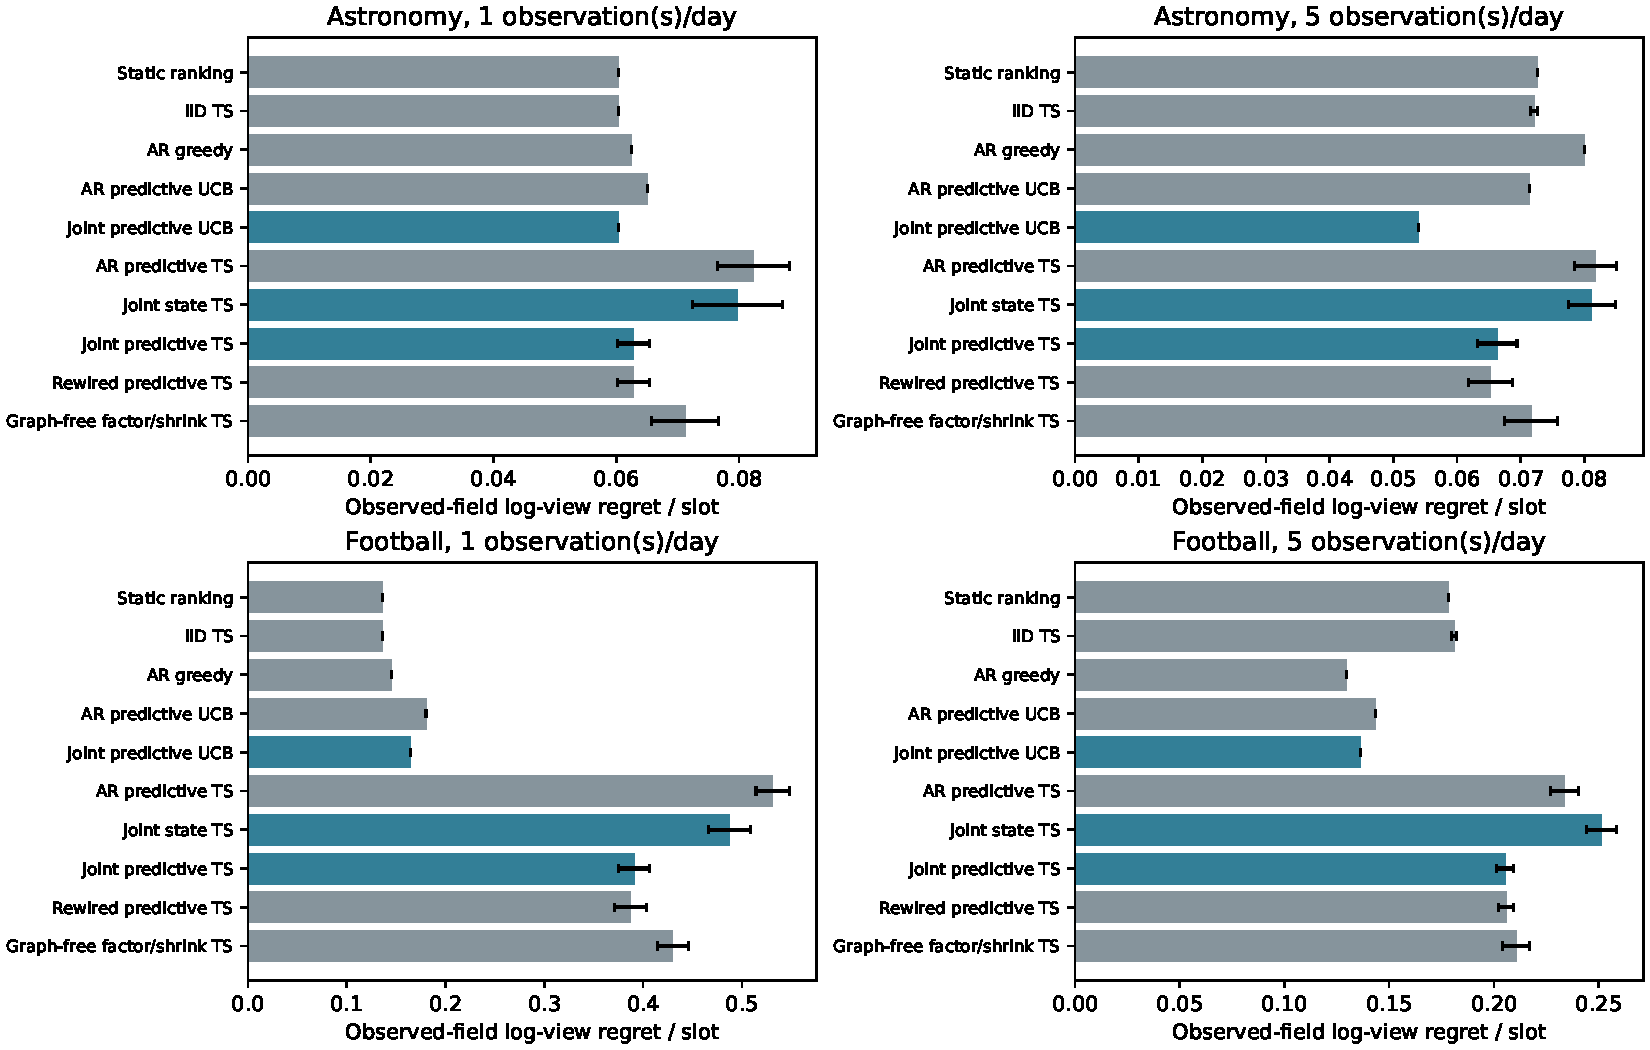
\includegraphics[width=\textwidth]{results/wikipedia/comparison.pdf}\caption{Completed Wikipedia AR(7) comparisons. Error bars are conditional 95\% Monte Carlo intervals over policy randomization on the same observed field; they are not population confidence intervals. Deterministic policies have no randomization interval.}\end{figure}

\begin{figure}[t]\centering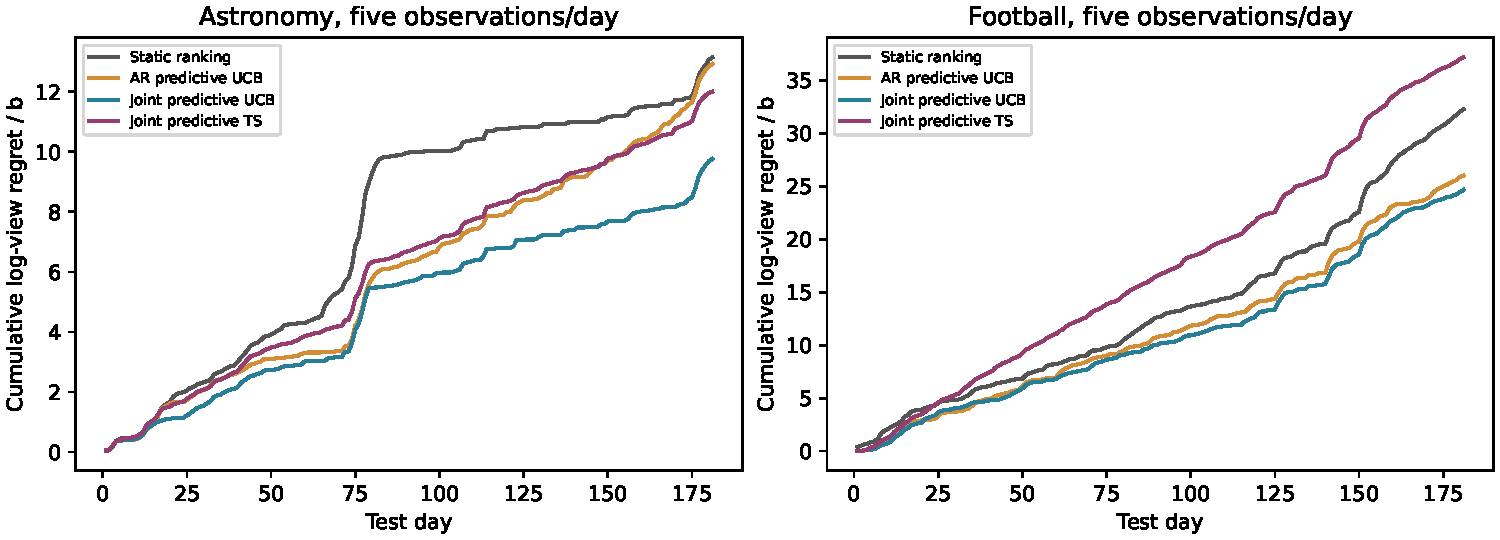
\includegraphics[width=\textwidth]{results/wikipedia/cumulative.pdf}\caption{Cumulative opportunity loss in the five-reading setting. One fixed test field per topic; no full-field test refresh is supplied to the learner.}\end{figure}

\subsection{What this application establishes}

A historical-graph, learned-general-AR selective-feedback study is feasible with a small data footprint and exact filtering. The outcomes also strengthen the negative controls: most apparent correlation benefit cannot be assigned to graph topology, and strong historical information can make simple static policies competitive. These conclusions are confined to two panels and the stated utility proxy. Raw-scale captured attention, conditional seed intervals, paired differences, monthly-block summaries, action traces and all fitted matrices are released; no theoretical floor or true stationary PCS is claimed for this real panel.


\section{Synthesis, practical implications and unresolved questions}

The results support objective-specific use of dependence. Persistent states can make a recently observed arm valuable for reward prediction while making its permanent mean difficult to identify. Correlated innovations can cancel in comparisons, but a graph that predicts permanent preferences need not predict transient shocks. The exact selected-history likelihood accounts for both effects without changing fixed physical means into a random population.

The strongest theoretical statements are conditional guarantees with explicit assumptions: graph-energy information geometry, predictable innovation regression, all-time fixed-mean confidence, correct stopping, a conservative mean-UCB bound, the current-oracle innovation floor, and exact restricted allocation cases. The strongest empirical statements are qualified by their designs: graph-free shrinkage accounts for much of KuaiRec's static gain; temporal modelling explains most of its daily pilot improvement; the fixed-truth AR(20) study shows different policy leaders for regret and selection; and the new Wikipedia evaluation tests learned general-AR models using genuinely historical graphs.

No graph benefit should be inferred from a joint-versus-iid comparison alone. The relevant test holds the temporal inference and decision rule fixed while comparing real topology with diagonal, common-factor, learned covariance and degree-preserving controls. A benefit in average prediction may also fail to change the top decision. Conversely, a small forecast improvement near a top-arm tie can have a useful decision effect.

Open theoretical questions include matching graph-and-time regret constants, finite-budget optimal contrast allocation, robust learned-model confidence, endogenous exposure and graph learning, and efficient long-horizon belief planning. Open application questions include identifying the actual observation cost, testing catalog births/deaths and drift, and validating whether measured attention is the intended business utility. Our public-data emulation provides counterfactual observed-field evaluation under selective masking; it does not constitute an online randomized platform deployment.

\section{Reproducibility and source provenance}

The package contains this manuscript, compiled PDF, editable sections, generated tables, raw Wikipedia API responses, historical revision identifiers and hashes, model matrices, daily action traces, per-run summaries, conditioning checks, and acquisition/run/analysis scripts. The evidence directory freezes compact source results and the five original technical derivations. Large original raw simulation runs are fingerprinted or linked rather than duplicated indiscriminately. The file \texttt{evidence\_manifest.json} records the source versions used in this synthesis.

The Wikipedia acquisition is sequential and cached, with an identifying user agent and rate-limit backoff. Page-view data use human traffic across access methods; missing dates are not filled with zero. Historical hyperlinks come only from revisions before 1 January 2024. The graph preserves isolated vertices and does not use current redirects to recover missing edges. Public attention data are CC0; revision material retains Wikipedia attribution/share-alike conditions and revision URLs.

The new experiment runs with one BLAS thread. Development is confined to 2024, and the final 2025 field is only exposed to the evaluation logger after each selected batch has been chosen. Code and source metadata disclose every fit, hyperparameter, privilege and numerical observation regularizer. Stochastic repeats quantify policy randomization on one realized panel, not population uncertainty across independent Web histories. The README supplies exact commands and a route for shrinking this reference manuscript into a venue-specific submission.
